\chapter{The HPS Detector}\label{chap:detector}

\begin{figure}
    \centering
    \includegraphics[width=0.85\textwidth]{figs/detector/detector.png}
    \caption{A 3D rendering of the HPS detector complete with the silicon vertex tracker (SVT), electromagnetic calorimeter (Ecal), and chicane.}
    \label{fig:detector}
\end{figure}

The Heavy Photon Search (HPS) is a precision vertexing experiment designed to measure both prompt and long-lived heavy photons that decay to $\epem$ pairs. The HPS detector is a compact, forward acceptance spectrometer with three main components - a silicon vertex tracker (SVT), an electromagnetic calorimeter (Ecal), and a three-magnet chicane. A rendering of the detector is shown in Fig. \ref{fig:detector}. The SVT is used to track particles and measure their  momentum, the Ecal is used for timing and triggering, and the analyzing magnet (the middle magnet of the chicane) bends charged particles for a momentum measurement and particle identification. 

The specific design of the detector components are optimized for the physics goals of HPS. To maximize the signal yield of $\aprime$s, particularly low mass and displaced $\aprime$s, the detector must have acceptance to small angles. The search for displaced vertices is limited by vertex resolution that is dominated by multiple scattering, thus the first layer must be placed as close to the target as possible.

Beam electrons that are elastically scattered in the target are the dominant source of background and can be eliminated with a selective trigger. The beam electrons that lose energy in the target due to Bremsstrahlung bend in the presence of the magnetic field and form the so-called ``wall of flame'' in the horizontal plane including the beam direction (referred to as the ``beam plane'') that would produce too much radiation damage in any detector component as shown in Fig. \ref{fig:beambg}. Thus, the SVT and Ecal are both split in top/bottom halves and placed as close to the beam plane as possible. In order to balance between maximizing signal yield, optimizing vertex resolution, and minimizing radiation damage, the detector is designed with a vertical opening angle of 15 mrad from the beam plane for both top and bottom halves.

The last major design consideration is due to the fact that beam gas interactions have potential to be a very significant background source increasing both detector occupancy and radiation damage. For this reason, the SVT and the space between the Ecal halves are under vacuum. In addition, there exist a possibility for a beam-gas interaction downstream of the target that will mock a downstream decay and look very signal-like. A medium-level vacuum ($10^{-5}$ Torr) is sufficient to mitigate these effects and as a result, all materials must be vacuum compatible (and are tested in a high vacuum test chamber). Lastly, all materials must be nonmagnetic because the SVT operates in a high magnetic field.

%there exist a possibility for a beam-gas interaction downstream of the target that will mock a downstream decay and look very signal-like. For this reason, the SVT and Ecal are under vacuum. As a result, all materials must be vacuum compatible (and are tested in a high vacuum test chamber). In addition, all materials must be nonmagnetic because the SVT operates in a high magnetic field.

\begin{figure}
    \centering
    \includegraphics[width=0.5\textwidth]{figs/detector/beam_bg.png}
    \caption{The rate of electrons in at the first layer of the SVT from the so-called ``wall of flame'' - beam electrons that lose energy due to bremmstrahlung in the target and bend in the magnetic field. To avoid the radiation damage from the wall of flame, the detector is split into top and bottom halves.}
    \label{fig:beambg}
\end{figure}

\section{The Continuous Electron Beam Accelerator Facility (CEBAF)}\label{sec:cebaf}

\begin{figure}
    \centering
    \includegraphics[width=0.85\textwidth]{figs/detector/cebaf.png}
    \caption{A schematic of the upgraded Continuous Electron Beam Accelerator Facility (CEBAF) at Jefferson Laboratory. The machine is a recirculating linear accelerator designed to send a beam of electrons of different currents and energies to four different experimental halls (Halls A - D).}
    \label{fig:cebaf}
\end{figure}

The high energy electron beam used for $\aprime$ production by bremstrahhlung on a thin target is provided by Jefferson Laboratory's Continuous Electron Beam Accelerator Facility (CEBAF) \cite{Kazimi:2013yua}. CEBAF is able to simultaneously deliver intense and energetic electron beams of different energies and currents to three different experimental halls (Hall A, Hall B, and Hall C). The recent upgrade allows for CEBAF to deliver beam to four experimental halls (an additional Hall D) in multiples of 2.2 GeV up to 12 GeV \cite{Burkert:2012rh} \cite{Dudek:2012vr}. Beyond and including the 2015 Engineering Run, HPS runs have all been in the 12 GeV era - that is with the upgrades.

CEBAF is a recirculating linear accelerator (linac) designed as a ``racetrack'' configuration where beam bunches are circulated multiple times through the same two linacs by arcs as shown in Fig. \ref{fig:cebaf}. Each cycle, or pass, around the accelerator adds an additional 2.2 GeV of beam energy for a maximum of 5 passes to Hall A, Hall B, and Hall C and an additional half pass to Hall D. Thus, the energy in a hall will be $0.1 \ \mathrm{GeV}+ n \times 2.2 \ \mathrm{GeV}$ for $n$ passes (the addition 0.1 GeV comes from the energy from the injector). CEBAF can deliver a beam current of up to 85 $\mu$A to halls A and C and deliver up to 5 $\mu$A to halls B and D (HPS utilizes a current far less than the maximum).

Electrons in the accelerator originate from the photoemission of a strained GaAs superlattice photocathode with an incident laser of 780 nm wavelength, which is equal to the band gap of the GaAs \cite{Maruyama:2004hx}. The incident laser is pulsed at 499 MHz for $\approx$ 40 ps. The photoemitted electrons are then brought to the the injector before finally entering the accelerator.

CEBAF accelerates electrons using superconducting radiofrequency (RF) cavities operating at 1500 MHz and by using an RF separator, can deliver beam pulses at either 500 MHz or 250 MHz, essentially a continuous duty cycle, to each of the four experimental halls. This short pulse time (2 - 4 ns) results in a near-continuous duty cycle and is essential to HPS as it reduces pileup effects while maximizing luminosity. The 12 GeV upgrade included a 750 MHz RF separator which allowed the beam to be diverted to the new Hall D.

\clearpage

\section{Hall B and HPS Beamline}\label{sec:beamline}

\begin{figure}
    \centering
    \includegraphics[width=0.85\textwidth]{figs/detector/hallb.png}
    \caption{A schematic of Hall B including the CLAS-12 spectrometer and the HPS detector in the Hall B alcove. The electron beam enters the hall from the left in this picture.}
    \label{fig:hallB}
\end{figure}

The HPS experiment is located in Hall B in an alcove behind the CLAS12 (CEBAF Large-Acceptance Spectrometer) detector, which is typically used for low-current precision nuclear physics. Hall B can receive either an electron or photon beam. In order to reduce pileup and beam background for the HPS experiment, the Hall B beam from CEBAF is a continuous beam structure with a bunch spacing at 2 ns (which is far shorter than the trigger window and comparable to the detector timing resolution).

The Hall B beamline begins with a large tagger dipole magnet which, when energized, steers the electron beam into the tagger dump below the beamline. The tagger magnet is far upstream of HPS and allows for tuning of the beam to an acceptable quality before delivering the beam to HPS. This is critical as the low acceptance of the tracker puts the silicon within 5 mm of the nominal beam plane even with the SVT fully retracted, thus a poor quality beam (one with a large spotsize, beam tails, or other instabilities) could cause unnecessary radiation damage to the detector. If a target is placed upstream of the tagger magnet, a photon beam can also be produced in Hall B which has been used for test runs for HPS in the past. The nominal configuration for HPS physics running is for the tagger magnet to be de-energized so that the electron beam can be delivered to HPS.

The beamline between the tagger magnet and HPS consists of several beam position monitors (BPMs) which measure the passing beam bunches to provide an estimate of beam current and position. A series of quadrupole magnets and horizontal and vertical correctors on the beamline are used for fast automatic correction to beam trajectories based on the BPM measurements. The quadrupole magnets are also used to squeeze the beam spotsize as small as possible at the target.

The Hall B beamline also includes several wire harps to measure the beam position and profile. These wire harps are composed of 2-3 thin metal wires connected to a motor; as the wires (which are at different angles to obtain both $x$ and $y$ profile measurements) traverse the beam profile, they will scatter beam particles resulting in an increase of the count rate of downstream halo counters. The rate of these counters is proportional to the beam intensity, thus a beam position and profile can be constructed with knowledge of the wire positions and halo counter rates. This is used for beam tuning as well as to ensure the beam is safe enough to perform wire scans with the wires directly connected to the SVT as described below. An example of a harp scan from the 2H02 harp, which is the closest wire harp to the HPS target at 2.2 m upstream, from the 2016 Engineering Run is shown in Fig. \ref{fig:harpscan}. The general strategy to achieve a small spot size at the target is to use the measurements from the 2H02 wire harp as well as several wire harps further upstream in conjunction with a series of quadrupole magnets along the beamline. The magnetic fields of the quadrupole magnets can be finely tuned such that the waist, that is the minimum beamspot size in the $y$-direction, is precisely at the target.

\begin{figure}
    \centering
    \includegraphics[width=0.5\textwidth]{figs/detector/2H02harp.jpg}
    \caption{An example of a scan from the 2H02 wire harp from the 2016 Engineering Run. This provides a measurement of the beam profile that is useful as in input to tuning the beam to its optimal profile at the target. The profile shows a width of 92 $\mu$m in $x$ and 14 $\mu$m in $y$ with minimal beam tails.}
    \label{fig:harpscan}
\end{figure}

There are several collimators along the beamline to protect both HPS silicon sensors and electronic components from radiation damage from a either a stray beam or particles produced by a stray beam. When enough of a beam interacts with a collimator, it also produces many particles that trip the fast shutdown (FSD). The closest collimator to the SVT is a 1 cm thick tungsten plate with machined slots of different widths connected to a linear shift and placed 2.9 m upstream of target (referred to as the ``SVT collimator''). With the exception of the inner strips of layer 1 of the SVT, this protects most of the detector from beam tails and beam halo. The collimator can also force an FSD trip such as when the beam is mis-steered or scrapes the collimator which can produce enough secondary particles for the FSD counters to cross threshold. For the 2016 Engineering Run, the 4 mm slot was used. 

\begin{figure}
    \centering
    \includegraphics[width=0.95\textwidth]{figs/detector/hpsbeamline.jpg}
    \caption{A schematic of the HPS beamline inside the Hall B alcove.}
    \label{fig:hpsbeamline}
\end{figure}

Downstream of HPS, there are two fluorescent screens and a screen used for optical transition radiation (OTR) that are useful for viewing the beam position. Finally, the beam is terminated in a Faraday cup in the Hall B beam dump. The Faraday cup provides the most accurate measurement of the total beam charge and is used to normalize the data for the analysis. A beam blocker must be put in front of the Faraday cup at beam currents above 50 nA to avoid overheating, and the actual measurement of integrated charge must be re-scaled.

A schematic of the HPS beamline in the Hall B alcove is shown in Fig. \ref{fig:hpsbeamline}. The HPS apparatus is a compact, forward spectrometer that consists of a three-magnet chicane system, SVT, Ecal, and a vacuum chamber. On the exterior of HPS, there are several halo counters (plastic scintillators) that monitor the stability of beam conditions. If these halo counters measure particle rates above their set threshold, most likely due to an obscured beam, a fast shut down (FSD) is applied to the Hall B beam within 1 ms to prevent further radiation damage to the HPS detector components.

Thin wires are attached to both top and bottom halves of the SVT as described in Sec. \ref{sec:svt_mechanical} and are used to measure the beam position and profile with respect to the SVT as close to the target as possible. Each half the SVT contains a horizontal and a diagonal wire (oriented $\approx 10^{\circ}$ from horizontal) for a vertical and horizontal position measurement. These wires move with the SVT and, as they traverse the beam profile, beam particles are scattered into the halo counters on the exterior of HPS. The rate of beam particles counted by the halo counters is proportional to the intensity of the beam, thus through a mapping of the wire position and count rate a beam profile can be produced. In order to ensure safe operation of the SVT, the beam profile in the $y$-direction is required have a width less than 50 $\mu$m with minimal beam tails and a mean within 50 $\mu$m of the midplane between the top and bottom halves of the SVT. However, a beamspot as small as possible is desired as a smaller spot size will aid the constraint of vertices to the beamspot, thus improving the displaced vertex analysis by more efficiently rejecting tracks and vertices that are inconsistent with the beamspot.  The beamspot size and position in the $x$-direction is less important since the resolution is far worse due to the the small stereo angles between the SVT strip sensors, so a width of less than 150 $\mu$m is sufficient. An example of a wire scan measurement from the 2016 Engineering Run is shown in Fig. \ref{fig:wirescan}.

\begin{figure}
    \centering
    \includegraphics[width=0.5\textwidth]{figs/detector/SVTwirescan.jpg}
    \caption{An example of an SVT wire scan measurement from the 2016 Engineering Run. This provides a measurement of the beam profile as close to the target as possible. This scan shows a beam with a 14 $\mu$m width in the $y$-direction with minimal tails and 35 $\mu$m from the nominal beam plane. This is an excellent beam profile for HPS.}
    \label{fig:wirescan}
\end{figure}

The SVT wire scans are unable to effectively measure the beam halo - beam electrons in the far tails of the Gaussian beam profile. This is important to understand for the purposes of long term radiation damage in the SVT. A measurement of beam halo from the 2015 Engineering Run by measuring occupancies in layer 1 of the SVT without the target is shown in Fig. \ref{fig:beamtails}. The beam halo intensity is $< 10^{-5}$ of the beam intensity which is sufficiently below the rate due to elastically-scattered beam electrons in the target, and thus is acceptable for HPS.

The chicane contains a single 18D36 analyzing magnet (or central magnet or pair spectrometer) with a pole length of 91.44 cm and a gap size of 45.72 $\times$ 15.24 cm$^2$. The analyzing magnet operated with a maximum field strength of 0.24 T for the 2015 Engineering Run and 0.50 T for the 2016 Engineering Run (the field strength scales linearly with beam energy and a maximum field strength of 1.5 T). In addition, two H-dipole Frascati magnets are set on either side of the analyzing magnet such that the total $\int \vec{B} \cdot \mathrm{d}\vec{l}$ for the chicane system is 0 (each Frascati magnetic has half the bending power of the analyzing magnet with opposite sign) which ensures the beam trajectory downstream of the chicane is independent of whether or not the chicane is powered. 

The vacuum box has flanges upstream of the analyzing magnet for penetration of linear motion systems, cooling lines, and power and signal cables. The HPS target can be moved remotely by a linear shift from a stepper motor on the vacuum flange and is cantilevered at a ceramic support rod. There are several target options that can be selected based on the linear position of the target mount - 4 $\mu$m tungsten (0.125\% radiation length design and 0.116\% radiation length measured), 8 $\mu$m tungsten (0.25\% radiation length design and 0.223\% radiation length measured), and a carbon target for calibration. The targets are connected to a grounding wire in order to prevent discharge due to charge buildup from the incident beam. The Ecal is downstream of the analyzing magnet. More details of the Hall B and HPS beamlines can be found in the HPS Beamline paper \cite{BALTZELL201769}.

\begin{figure}
    \centering
    \includegraphics[width=0.5\textwidth]{figs/detector/beamtails.jpg}
    \caption{A measurement of the beam halo from 2015 Engineering Run using the occupancy of the first layer of the SVT in a no target run. The beam halo shows a with of 960 $\mu$m and 5 orders of magnitude less than the peak of the beam.}
    \label{fig:beamtails}
\end{figure}

\clearpage

\section{Silicon Vertex Tracker}\label{sec:svt}

\begin{figure}
    \centering
    \includegraphics[width=0.85\textwidth]{figs/detector/svt.png}
    \caption{A schematic of the HPS silicon vertex tracker (SVT) which includes 6 layers of silicon microstrip sensors inside a vacuum and a uniform magnetic field.}
    \label{fig:svt}
\end{figure}

The silicon vertex tracker (SVT) provides a momentum measurement from charged particle trajectories that bend in the uniform magnetic field and can be used to reconstruct a vertex position. The SVT is an array of silicon microstrip sensors consisting of six layers (or measurement stations). Microstrips provide a 1D measurement along the direction of the sensor extending away from the beam. In order to provide a 3D measurement, each layer contains two components - an axial sensor with strips parallel to the beam plane and a stereo sensor rotated at a small angle. A large stereo angle would provide improved hit resolution in the direction along the axial strip, and hence improved momentum resolution.\footnote{The resolution in the bend plane is simply the resolution in the non-bend plane divided by the stereo angle.} However, a large stereo angle would also cause the stereo sensors to dip significantly into the beam plane, lose acceptance, and be prone to ghost hits (falsely reconstructed 3D hits). In addition, since resolution effects are limited by multiple scattering, improving resolution in the $x$ direction by increasing the stereo angle is not necessary. Thus, the stereo angle is intentionally small and designed to be 0.100 mrad for the first three layers and 0.050 mrad for the last three layers. The axial/stereo sensor pairs reconstruct a 3D hit position at each of the six layers that are used for track finding. The difference in stereo angle between the first and last three SVT layers breaks the degeneracy in pattern recognition that could have generated more ghost hits. %to provide a compromise between these affects and hit resolution. The axial/stereo sensor pairs reconstruct a 3D hit position at each of the six layers that are used for track finding.

The SVT is split into top/bottom halves to avoid the very high flux of electrons near the beam plane due to the ``wall of flame". Both the top and bottom halves are designed at a 15 mrad opening angle with respect to the primary interaction point. This opening angle must be as small as possible in order to capture as many $A'$s as possible which are typically highly boosted with a small opening angle.\footnote{This becomes even more critical for displaced $A'$s which, for a given opening angle, lose acceptance rapidly as the decay vertex increases along the beam direction.} The last three layers of the SVT are double wide (i.e. two sensors end to end) to increase acceptance for charged particles that are bending due to the uniform magnetic field.

The six layers are arranged such that the distance between the first and second layer (layer 1 and layer 2) and the second and third layer is about 10 cm. The distance between the remaining layers is about 20 cm. Layer 1 is placed as close to the target as possible at about 10 cm in order to provide the best possible vertex resolution, and subsequently the second layer is placed close to the first layer to maximize pointing resolutions of tracks back to layer 1. The limiting factor of the first layer placement is the fact that the sensors cannot be closer to 500 $\mu$m from the beam plane in order to avoid significant radiation damage from both elastically scattered electrons in the target and beam tails. Thus for a given opening angle of 15 mrad and a 1 mm guard ring (inactive silicon) where the active sensor begins at $0.5 + 1.0 \ \mathrm{mm}= 1.5 \ \mathrm{mm}$, the closest the first layer can be placed downstream of the target is $\sim$1.5 mm / 15 mrad = 10 cm.\footnote{The next subsection describes a 1 mm inactive part of the sensor, so the active region begins at 1.5 mm from the beam plane.} This approaches the maximum allowed occupancy for the silicon sensors of $\sim 1-2$\%. The sensors are designed to be as thin as possible to reduce the material budget and hence the effects due to multiple scattering. A summary of the some of the important design features of the SVT is shown in Table \ref{tab:svt}.

\begin{table}[!hb] 
    \centering
    \begin{tabular}{lcccccc}
        \toprule
        \textbf{Layer Number} & \textbf{1} & \textbf{2} & \textbf{3} & \textbf{4} & \textbf{5} & \textbf{6} \\
        \midrule
        \midrule
            Distance $z$ from target (mm) & 100 & 200 & 300 & 500 & 700 & 900 \\
            Dead Zone Distance $y$ (mm) & $\pm$1.5 & $\pm$3.0 & $\pm$4.5 & $\pm$7.5 & $\pm$10.5 & $\pm$13.5 \\
            Number of Sensors & 4 & 4 & 4 & 8 & 8 & 8 \\
            Stereo Angle (mrad) & 100 & 100 & 100 & 50 & 50 & 50 \\
            Bend Plane Resolution ($\mu$m) & $\approx$ 60 & $\approx$ 60 & $\approx$ 60 & $\approx$ 120 & $\approx$ 120 & $\approx$ 120 \\
            Non-Bend Plane Resolution ($\mu$m) & $\approx$ 6 & $\approx$ 6 & $\approx$ 6 & $\approx$ 6 & $\approx$ 6 & $\approx$ 6 \\
            Material Budget (\%$X_0$) & 0.7\% & 0.7\% & 0.7\% & 0.7\% & 0.7\% & 0.7\% \\
            Module Power Consumption (W) & 6.9 & 6.9 & 6.9 & 13.8 & 13.8 & 13.8 \\
        \bottomrule
    \end{tabular}
    \caption{A summary of the basic parameters for different layers in the SVT.}
    \label{tab:svt}
\end{table}

\clearpage

\subsection{Sensors and Readout}\label{sec:sensors}

\begin{figure}
    \centering
    \includegraphics[width=0.5\textwidth]{figs/detector/apv25.png}
    \caption{A schematic of the APV25 deep submicron readout chip that was originally designed for CMS detectors but is used for the HPS SVT.}
    \label{fig:apv25}
\end{figure}

HPS utilizes the silicon microstrip sensors originally designed and procured for the upgraded D\O \  detector at Fermilab for run IIb, which was cancelled in favor of an insertable Layer 0 \cite{D0Collab:2003}. The sensor technology was chosen to minimize material budget to mitigate multiple scattering effects and to be highly tolerant to radiation. These sensors are single-sided p+n with AC-coupled readout with a bulk that is lightly doped n-type silicon. The strip implants are strongly p-type doped. The bias of the strips comes from polysilicon resistors at the end of the strips which are capacitively coupled to aluminum readout strips that run on top of the silicon strips.

The sensor cut dimensions are 100 mm $\times$ 40.34 mm with an active area of 98.33 mm $\times$ 38.34 mm. The silicon strip pitch is 30 $\mu$m; however, only every other strip is readout (i.e. the readout pitch is 60 $\mu$m). When a particle is incident on an intermediate strips (a sense strip), the charge will split between the neighboring readout strips and this charge sharing will improve single hit resolution. Each sensor has 640 readout strips.

The useful sensor lifetime is limited by radiation damage where the sensor strips closest to the beam plane are expected to undergo a large electron flux of $>10^{15}$ electrons per cm$^2$ over the duration of the experiment. Specifically, incident particles can displace silicon nuclei from their crystal lattice which causes an effective type inversion, where the n-type bulk is converted to p-type. The radiation damage leads to an increase in depletion voltage which means the charge collection efficiency for a given bias voltage will decrease. Thus as a sensor undergoes radiation damage over the course of the run which is highly non-uniform and concentrated on the beam edge of the sensor (mostly from beam electrons elastically scattered in the target), the bias voltage must be increased to keep the same charge collection efficiency. Eventually, this bias voltage will approach the breakdown voltage and will no longer be usable in the experiment. In addition, radiation damage leads to increased leakage current, and thus sensor heating. For these sensors, the nominal operating bias voltage is 180 V. The design specifications required a breakdown voltage greater than 350 V; however, only sensors with a breakdown voltage greater than 1000 V were used. For the 2015 and 2016 Engineering Runs, radiation damage was not an issue. 

These sensors are readout by the APV25 readout chip which was developed for the silicon microstrip sensors in the CMS tracker \cite{Raymond:2000ey} \cite{French:2001xb}. A schematic is shown in Fig. \ref{fig:apv25}. The APV25 chip has high hit time resolution and has the ability to readout multiple consecutive samples of its shaper waveform, thus it is useful for pileup rejection - an essential requirement for HPS. The APV25 chip has 128 input channels, thus each sensor has 640 / 128 = 5 readout chips. Each channel contains a charge-sensitive preamplifier with an optional inverter, CR-RC shaper, and a 192-cell-deep analog pipeline. Only 160 out of 192 of these cells are used to buffer samples and the remaining 32 cells buffer the addresses of samples waiting to be readout. A picture of two SVT sensors with APV25 chips is shown in Fig. \ref{fig:sensor}.

\begin{figure}
    \centering
    \includegraphics[width=0.95\textwidth]{figs/detector/sensor.png}
    \caption{A picture of the two SVT sensors (end to end). The sensors are readout by APV25 chips which are housed on a hybrid circuit. }
    \label{fig:sensor}
\end{figure}

The clock is designed for a clock period of 25 ns which is equivalent to the LHC bunch crossing. However, HPS adapted this chip to run on a clock period of 24 ns (41.6 MHz) since it is an even multiple of the both the JLab and Ecal clocks, which are 2 ns and 4 ns, respectively. Each channel samples the shaper output and stores it in a cell of its pipeline on each clock. Once a trigger is received, the pipeline cell of each channel is readout, and the chip multiplexes the 128 signals onto a single differential current output. A configurable latency (the distance between the read and write pointers) setting determines which pipeline cells are readout. 

The samples are readout by the Analog Pulse Shape Processor (APSP) which has the ability to operate in two distinct modes - deconvolution mode and multi-peak mode. For each trigger signal, the deconvolution mode allows for three consecutive pipeline cells to be readout and combined into a weighted sum whereas the multi-peak readout mode allows for three consecutive pipeline cells to be readout without any additional operations. In order to mitigate pile-up effects from large occupancy, HPS is operated in multi-peak readout mode and for each trigger, the APV25s are sent two consecutive trigger signals for a total of six samples. These six samples are fit to a pulse shape predetermined from offline calibration and reconstructed offline in order to obtain the pulse amplitude and hit time. This is described in detail in Sec. \ref{sec:svtrecon}.

During the 2015 Engineering Run, the nominal settings of the APV25 were utilized. For the 2016 Engineering Run, these same parameters were used with the exception of the input parameters of the pulse shaper which were optimized to have a sharp rise time for optimal time resolution and quick fall time to further reduce pileup effects. A schematic of the APV25 shaper and the parameters which were optimized is shown in Fig. \ref{fig:apv25shaper}.

%isha = n times 1 mu A for (0,255)
%VFS = -1.25 V - 7.5 mV x n (0,255)

%Nominal settings are isha = 34 and VFS = 60
%Optimal settings are isha = 70 and VFS = 0
%\textcolor{red}{Include pulse shaper optimization plots?}

\begin{figure}
    \centering
    \includegraphics[width=0.5\textwidth]{figs/detector/apv25shaper.png}
    \caption{A schematic of the APV25 Shaper. The parameters VFS (related to the input voltage) and isha (related to the input current) were optimized for improved time resolution and reduced pileup.}
    \label{fig:apv25shaper}
\end{figure}

\clearpage

\subsection{SVT Mechanics}\label{sec:svt_mechanical}

\begin{figure}
    \centering
    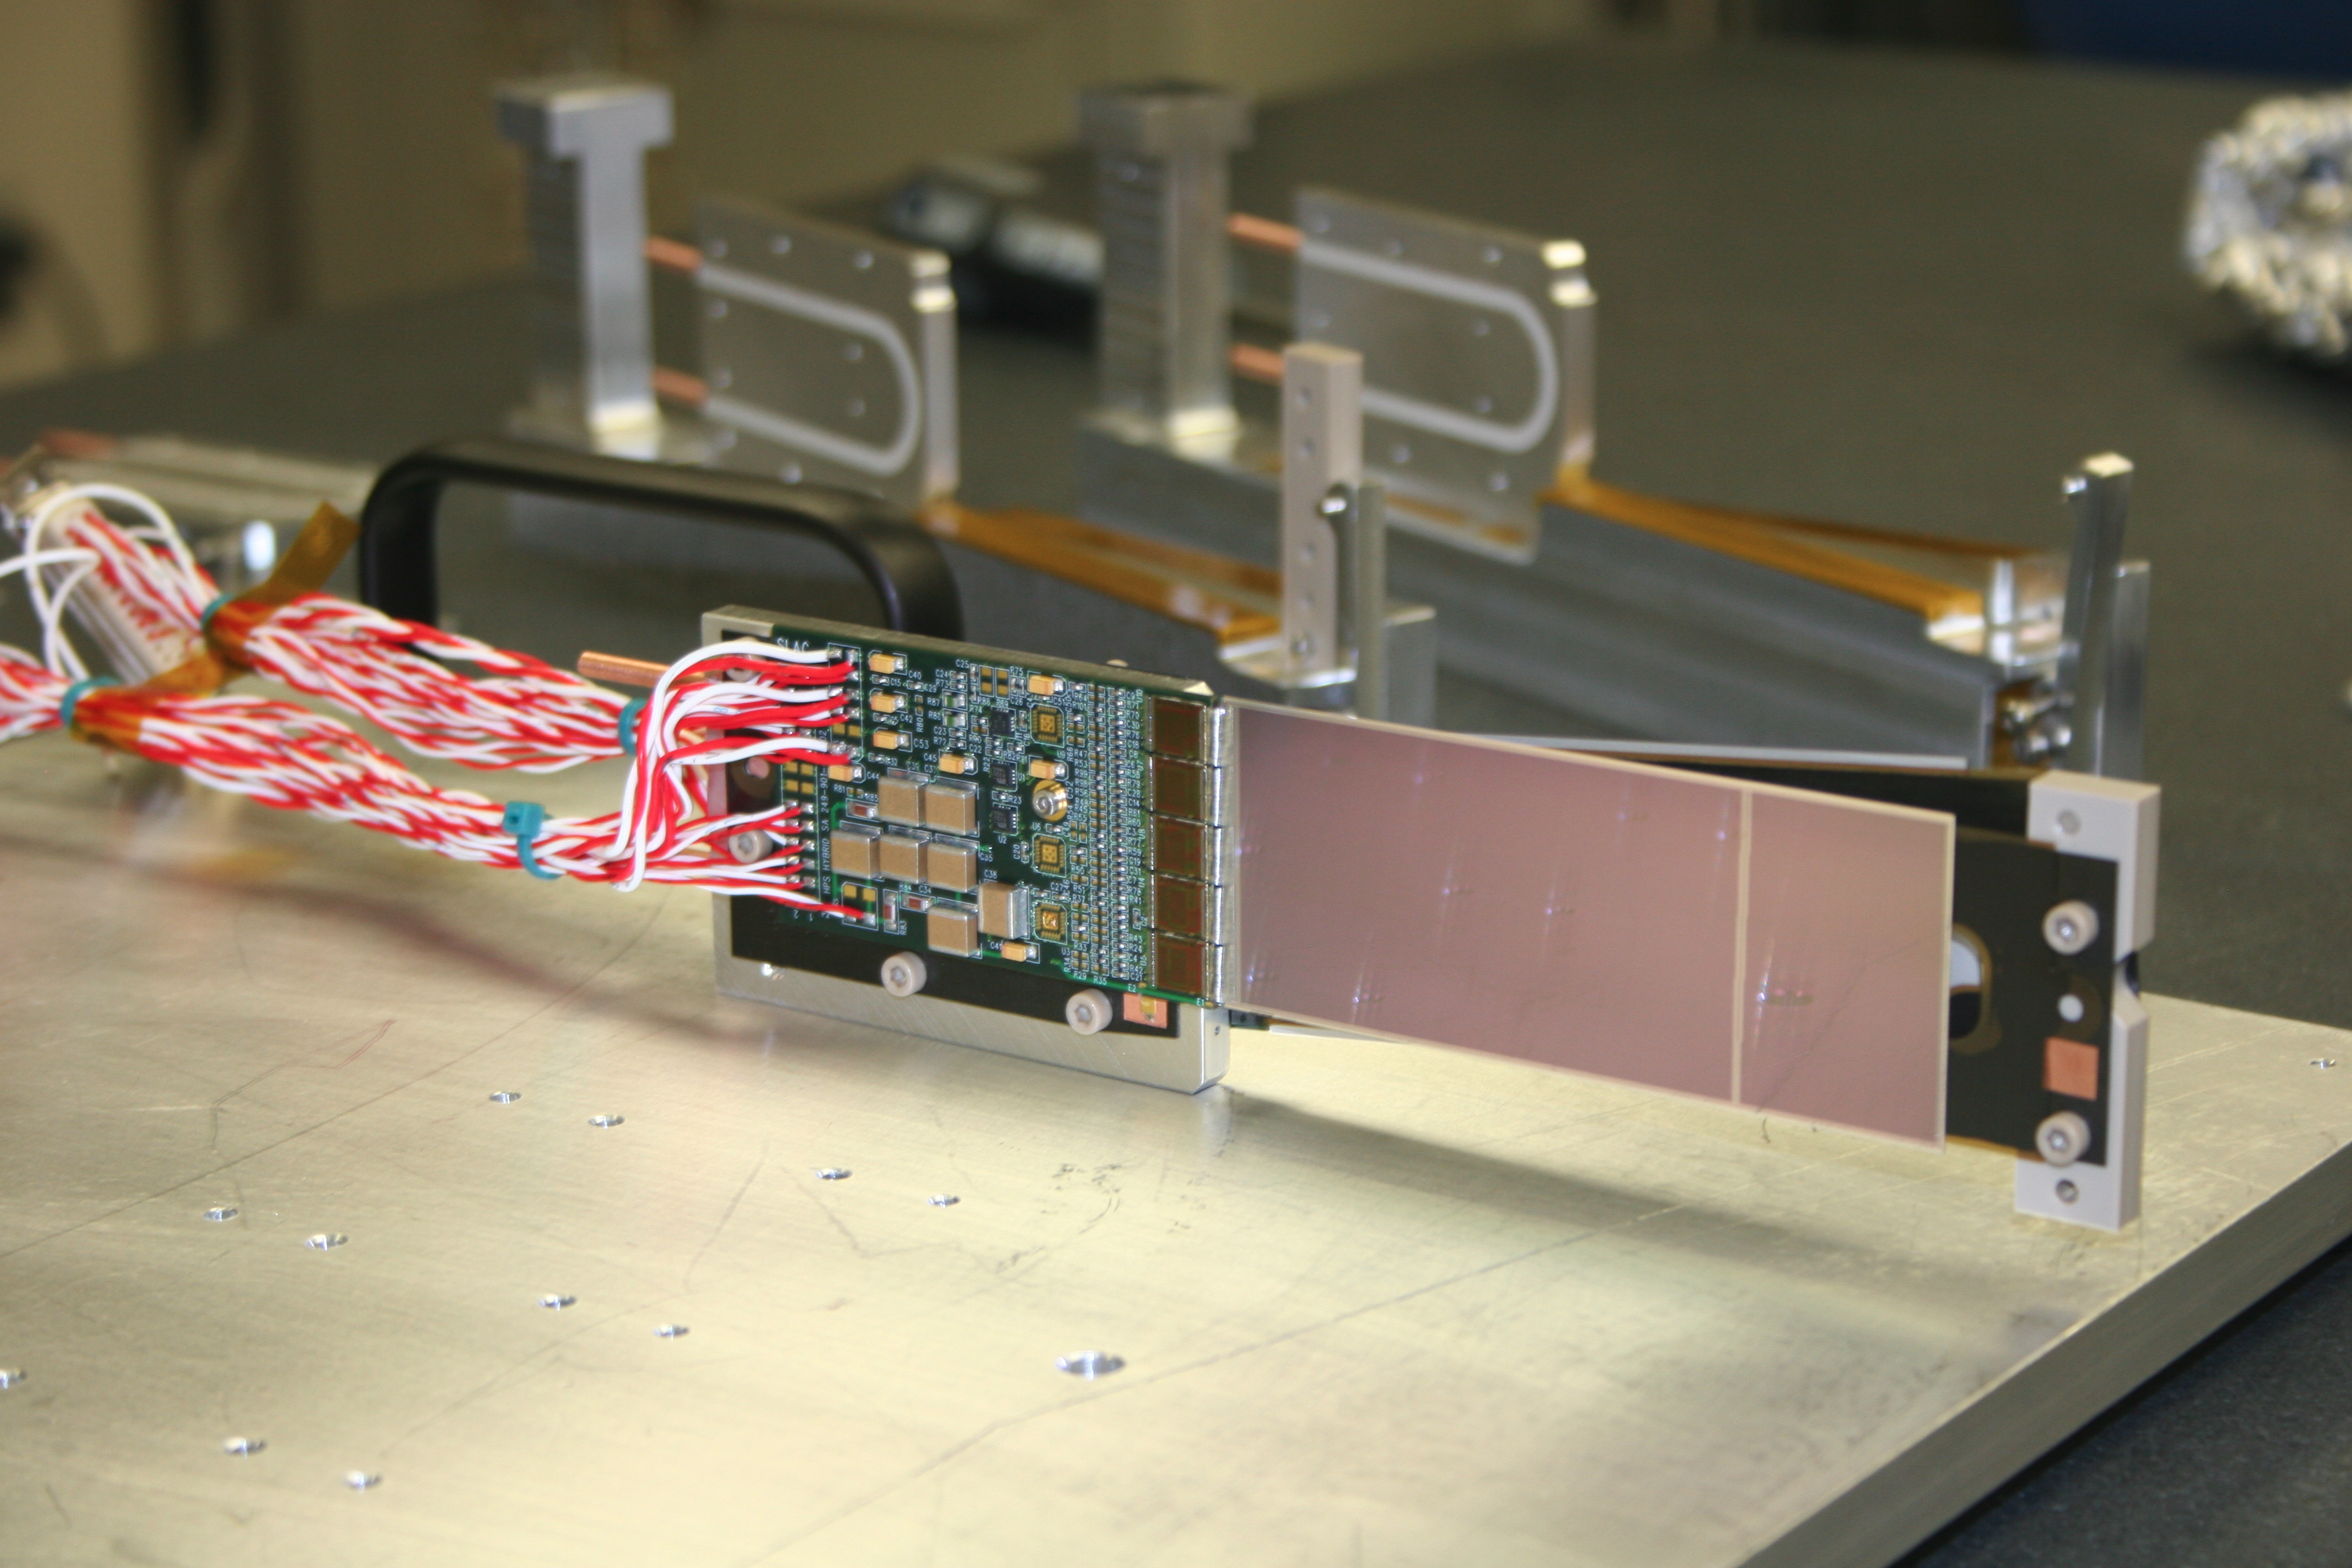
\includegraphics[width=0.5\textwidth]{figs/detector/module.png}
    \caption{A single SVT module which comprises of two silicon microstrip sensors which are axial (front) and stereo (back) to the beam plane. Each sensor is supported by a carbon fiber support structure can be seen protruding from the right of the axial sensor.}
    \label{fig:svtmodule}
\end{figure}

Each sensor is part of a base unit referred to as a ``half-module" and is comprised of a single or double sensor, carbon fiber support structure, and hybrid readout circuit boards. The first three layers 1-3 are composed of a single sensor and hybrid while the last three layers 4-6, since they are double wide, are composed of double sensors and hybrids. Each of these half-modules can be used as the axial or stereo components of the detector.

The carbon fiber, in addition to support for the sensor, acts as ground plane for the half-module while a layer of Kapton insulation isolates the carbon fiber from the back of the sensor which is at high voltage. The Kapton and carbon fiber are kept as thin as possible, much thinner than the silicon sensors, to avoid adding additional unnecessary material that increases multiple scattering in the tracker.\footnote{A window was machined into the carbon fiber support such that the material in the middle of the sensor, where most of the physics of interest is expected, is further minimized.}

The hybrid circuit boards house the APV25 readout chips, five per half module, and provides a connection of the sensor to the rest of the DAQ. The APV25 power, control lines, and output channels are wirebonded to the hybrid while the input channels are wirebonded directly to the sensor. The hybrid contains temperature sensors and carries filter capacitors for the sensor bias.

Two of these half-modules are paired to create a module with one axial and one stereo half-module. The axial half-modules are parallel to the beam plane and the stereo half-modules are rotated at a small angle and dips into the beam plane on the positron side (beam left, the side opposite to where beam background is bent). These modules are mounted on aluminum support modules which hold the half-modules from both sides and, in addition to mechanical support, these supports also pull heat generated by the hybrids. The half-modules and the support undergo thermal contraction at different rates, thus the module support applies a constant tension from a spring pivot in order to keep the half-modules flat at operating temperature ($\sim 0^{\circ}$ C). A picture of a complete module is shown in Fig. \ref{fig:svtmodule}.

Three of these modules are mounted on an aluminum support structure called a ``U-channel". The SVT contains a total of four of these U-channels for each top and bottom of L1-3 and L4-6 (which are larger). Each U-channel is supported by kinematic mounts which guarantee reliable and repeatable positioning when the U-channels are installed and re-installed. The L1-3 U-channels rest on two downstream kinematic mounts, which act as a hinge, and is supported at the upstream end by motion levers which guide the L1-3 U-channels towards and away from beam. Finally, the L1-3 modules house scan wires as close to the target position as possible to measure the beam position and profile relative to the SVT to assess beam quality. Each U-channel has two wires - one parallel to the beam plane and one rotated at a slight angle - in order to obtain 2D position information. A picture of a L1-3 U-channel is shown in Fig. \ref{fig:uchannel}.

\begin{figure}
    \centering
    \includegraphics[width=0.5\textwidth]{figs/detector/U1-3.png}
    \caption{Layers 1 - 3 modules of the SVT (from left to right) are place in one of the U-channels. Copper cooling lines and electrical lines can be seen. The wire frames and scan wires can also be seen on the left.}
    \label{fig:uchannel}
\end{figure}

The SVT underwent a mechanical survey before installation using a coordinate-measuring machine which utilized both optical and touch probe measurements to locate 3D target points. The survey ensures the SVT was assembled as designed and allows adjustment for the adjustable components if necessary, and it provides an initial alignment for track reconstruction whose quality depends strongly on precise knowledge of the sensor positions and orientations. This is sufficient for initial knowledge, but the sensor is later aligned using the data as described in Sec. \ref{sec:alignment}. Lastly, the survey provides a measurement of the edge of the L1 axial sensor relative to the wire on the U-channel to ensure that the sensor edge is placed at 500 $\mu$m from the beam plane. A picture of the SVT installed in the SVT vacuum box is shown in Fig. \ref{fig:svtvaccum}.

\begin{figure}
    \centering
    \includegraphics[width=0.95\textwidth]{figs/detector/vacuumbox.png}
    \caption{A picture inside the SVT vacuum chamber with everything installed except for the target. The frontend boards (FEBs) and FEB cooling plate are on the left. The SVT cooling lines protrude outward in the picture. The first layer of the SVT can be seen in the back behind the wire frames. The SVT is in its closed position and the beam must go through the 1 mm gap between the top and bottom sensors.}
    \label{fig:svtvaccum}
\end{figure}

%A coordinate-measuring machine uses both optical and touch probe measurements to locate 3D target points. The touch probe has higher precision in general so it is used whenever possible, though the optical measurement must be made on the silicon sensors themselves. Several different measures are made. First, individual sensors are measured with respect to . Finally, the fully assembled U-channels are measured as a cross-check with the other measurements...

\clearpage

\subsection{SVT Data Acquisition, Power, and Services}\label{sec:svt_daq}

\begin{figure}
    \centering
    \includegraphics[width=0.5\textwidth]{figs/detector/svt-daq-schematic.png}
    \caption{A schematic of the SVT DAQ system described in Sec. \ref{sec:svt_daq}.}
    \label{fig:svtdaq}
\end{figure}

HPS must have a method to pass power and data to the detector given the constraints of the detector design as described previously. In addition, the nearest rack that can contain the data acquisition (DAQ) and power supplies is located about 20 m from where HPS is installed thus requiring the analog signals from the APV25 readout chips to be converted to optical digitized signals. As a result, the signal digitization and low-voltage regulation is performed inside the vacuum on front end boards (FEBs) located on a cooling plate alongside the SVT. And because the SVT and front end boards (FEBs) are in vacuum, all power and DAQ must pass through a pair of 8-inch vacuum flanges upstream of the dipole magnet, thus requiring the reduction of the number of signals.

Each of the 10 FEBs can service either a pair of L1-3 modules or a single L4-6 modules totalling four hybrids which is connected by a single bundle of impedance-controlled twisted pair magnet wire (which reduces crosstalk and electromagnetic interference between the lines). This carries the analog APV25 output signals, digital controls, trigger signals, low-voltage power, and high-voltage sensor bias. The data and control signals are carried by a mini-SAS cable on a high-speed data link. The FEBs digitize the output signals from 20 APV25 chips (4 hybrids $\times$ 5 APV25 chips). A preamplifier on the APV25 converts a differential current signal to voltage and is digitized to a value between 0 and 16384 by an AD9252 14-bit analog to digital converter (ADC) which samples the signal at 41.667 MHz.\footnote{The 14-bit samples for each of the 23040 APV25 channels is too much data to store. The DAQ requires a readout threshold of three out of six samples above a threshold (three times the channel noise above the mean) that is predetermined from offline calibration.} Each FEB contains a Xilinx Artix-7 FPGA that sends the ADC data upstream to multi-gigabit receivers and controls and monitors the hybrid state and configuration.

%FEBs also distribute low-voltage power to the hybrids by supplying a single voltage by splitting into four independent voltages and using a combination of switching and linear voltage regulators. Improves noise performance, reduces number of voltages that must be passed through vacuum chamber. High-voltage is also passed, but directly.

The digitized data, low-voltage power, and high-voltage bias from the FEBs is transferred to electronic boards on the penetration of the vacuum flange (called ``flange boards'') through mini SAS cable for data and twisted pair cables for power and bias.\footnote{The flange boards are custom-made since the number of required connections is too high for conventional vacuum feedthroughs.} There are two flange boards on the beam right side - one for high voltage and the other for low voltage. The four flange boards located on the beam left side convert the digitized signal to optical using fiber transceivers so the signal can be transferred a large distance to the general-purpose Reconfigurable Cluster Elements (RCE) platform. The RCE platform was developed at SLAC and is housed in a standard Advanced Telecommunications Computing Architecture (ATCA) crate. The data from the FEBs is distributed on a Cluster on board (COB) between two ATCA blades housed inside the crate. Each COB contains 8 RCE processing nodes which use Xilinx Zynq-7000 series FGPAs to apply data reduction to signals from the flange boards and build events.

Each COB houses several generic hardware daughterboards common to RCE platforms including four Data Processing Modules (DPM) and one Data Transport Module (DTM). The DPMs process and reduce data at high speed while the DTM is responsible for timing and trigger distribution. The only HPS-specfic hardware on the COB is the Rear Transition Module (RTM) which interfaces the optical fibers from the signal flange boards to the COB. The SVT DAQ utilizes a total of two COBS and two RTMs. In addition to the core of the DAQ, the rack also contains the low and high voltage Wiener MPOD power supplies which are commonly used for a variety of JLab experiments. A schematic of the SVT DAQ system is shown in Fig. \ref{fig:svtdaq}.

The SVT services - motion, cooling, and power - are supplied from outside the vacuum through several flanges located upstream of the vacuum chamber. The SVT is cooled through two independent cooling loops - one for the silicon sensors and the other for the FEBs. The silicon sensors must be kept below 0$^{\circ}$ C in order to avoid further radiation damage due to higher temperature (called reverse annealing). They are cooled through a hydrofluoroether compound circulating through copper lines embedded into the U-channels where the top and bottom are split and L1-L3 and L4-L6 are connected in series. The specialized fluid is necessary since its low viscosity maintains high flow rates at low temperatures.

%The FEBs only need to be kept at around room temperature while dissipating only the heat the produced from operating the FEBs themselves. 
Only the heat produced from operating the FEBs themselves needs to be dissipated. Thus, distilled water is sufficient as a cooling fluid and is circulated through copper lines embedded in the FEB cooling plate. The FEBs themselves are cooled through direct thermal contact with the cooling plate. A picture of the FEBs on the cooling plate is shown in Fig. \ref{fig:FEBcooling}.

\begin{figure}
    \centering
    \includegraphics[width=0.5\textwidth]{figs/detector/FEBcooling.png}
    \caption{The FEB cooling plate complete with 10 FEBs fastened to the front and back of the plate.}
    \label{fig:FEBcooling}
\end{figure}

In addition to cooling components, there are three linear shift stepper motors that provide independent motion control of the top and bottom U-channels as well as the target frame. The motors are powered and controlled by a Newport XPS controller. All three motors have both a hardware and software safety stop, while the two motors that control the U-channel linear motion also include a precision limit switch to ensure the SVT is not accidentally driven into the beam.

\clearpage

\section{Electromagnetic Calorimeter and Trigger}\label{sec:ecal}

\begin{figure}
    \centering
    \includegraphics[width=0.85\textwidth]{figs/detector/ecal.png}
    \caption{A rendering of the beam's eye view of the HPS Ecal. Each segment is one of the 442 lead tungstate crystals and the Ecal is split in half to avoid radiation damage from the most intense parts of the beam.}
    \label{fig:ecal}
\end{figure}

The electromagnetic calorimeter (ECal) is an array of 442 lead tungstate scintillating crystals (PbWO$_4$) and is used primarily for precision timing and triggering \cite{Balossino_2017}. The crystals are reused from the CLAS Inner Calorimeter (IC). The crystals have front faces of size 1.3 $\times$ 1.3 cm$^2$, are 16 cm long, and are tapered such that the back faces have dimensions 1.6 $\times$ 1.6 cm$^2$ for acceptance purposes. The Ecal itself is split into top and bottom halves much like the SVT to avoid the most intense parts of the beam plane. Each half contains 5 rows of 46 crystals with the exception of the removal of 9 crystals in the innermost row to avoid large occupancy from beam background. This is referred to as the Ecal hole or electron gap. The innermost rows are positioned 2 cm from the beam plane to maintain the 15 mrad design opening angle. The face of the Ecal is positioned 139.3 cm from the target position. Scintillation light from each crystal is detected by an avalanche photodiode (APD) on the back face of the crystal (specifically, a Hamamatsu S8664-1010 APD). One blue and one red LED are positioned on the front face of each crystal and are used for monitoring purposes (specifically radiation damage and stability of readout gain). Since the scintillator response is temperature-dependent, the Ecal is surrounded by a thermal enclosure.

The primary purpose of the Ecal is to trigger the experiment. Jefferson Laboratory has developed general-purpose readout boards called the FADC250 digitizer boards, or simply FADC. APD signals are amplified by a preamplifier that outputs signals through a motherboard. Each FADC board has 16 input channels and are continuously digitized at 250 MHz to a 12-bit precision which are then stored in 8 $\mu$s deep pipelines to await being readout if a trigger signal is received. There are several readout modes available, but HPS utilizes the readout mode that outputs a window of 100 samples that allows pulse fitting with optimal time resolution.

\begin{figure}
    \centering
    \includegraphics[width=0.85\textwidth]{figs/detector/ecal_crystal.png}
    \caption{A schematic of a PbWO$_4$ crystal in the Ecal.}
    \label{fig:ecalcrystal}
\end{figure}

The FADC boards are located in VXS crates also developed by Jefferson Laboratory as a general-purpose trigger framework. An algorithm that continuously looks for threshold crossings and integrates the digitized signal from the FADC within a fixed window converts the integration to an energy from previously calibrated values from cosmic rays. This gives a crystal position, energy, and time of the threshold crossing which are then passed to the Global Trigger Processor (GTP) every 32 ns. Each Ecal half has a GTP board which clusters hits by looking at a 3 $\times$ 3 block around a center crystal with at least 50 MeV and the surrounding hits within 16 ns of the center hit. This defines a cluster with a center crystal, hit time, number of hits, and total energy. Each GTP reports these clusters to the Single Subsystem Processor (SSP) board.

The SSP uses these clusters to make a decision on the Trigger. For the 2016 Engineering Run, there were a total of 5 triggers utilized. The first is a ``pulser'' trigger which fires at a fixed rate of 100 kHz. Next, there are two triggers that fire on single clusters that are called ``singles1'' and its corresponding trigger which has looser requirements ``singles0''. Finally, there are two triggers that fire on a pair of top-bottom clusters (at least one cluster in each GTP). These are called ``pairs1'' and ``pairs0'' triggers, where pairs0 is the looser version of pairs1. The pairs1 is our nominal trigger that is used for the physics analysis. In order to prevent the other triggers from triggering at a rate higher than the DAQ can handle, the singles triggers and the pairs0 trigger are prescaled such that one trigger in $2^n$ triggers are accepted where n is in the range of 10 to 13.

Once the SSP makes a trigger decision, if a cluster or pair of clusters meets the requirements above a trigger is sent to the Trigger Supervisor board (TS) and distributes the trigger to the Trigger Interface (TI) boards. The TS can reject the trigger if a subsystem is not ready to accept a trigger or the trigger follows too closely to another trigger.

The livetime of the DAQ, that is the fraction of time the DAQ is willing to receive triggers, must be understood in order to properly normalize the data. One way to measure the livetime is to use the pulser trigger. Since the pulser trigger fires at a constant rate, the ratio of the number of pulser triggers recorded to the number of pulser triggers that should have been recorded based on the 100 Hz rate is a direct measurement of the livetime. Another way to measure the livetime is to combine the measurement of integrated charge from the Faraday cup as described in Sec. \ref{sec:beamline} with a measurement of the integrated charge with the DAQ live. This is called the ``gated Faraday cup scaler'', and the ratio of this scalar to the total integrated charge is the DAQ livetime.

\begin{figure}
    \centering
    \includegraphics[width=0.85\textwidth]{figs/detector/ecal_trigger.png}
    \caption{A schematic of the trigger for the Ecal. Top and bottom halves of the Ecal are each are readout by FADC readout boards, and then sent to the SSP where a trigger decision is made.}
    \label{fig:ecaltrigger}
\end{figure}

The HPS physics trigger is designed to maximize efficiency for $A's$, or more generally $\epem$ pairs near the beam energy, while sufficiently suppressing backgrounds to avoid overwhelming the DAQ systems. The most significant one-cluster background is electrons elastically-scattered in the target. Thus a trigger requiring at least two clusters will eliminate a large fraction of these. The largest source of two-cluster backgrounds is wide-angle bremsstralung (WABs) in coincidence with a beam electron elastically scattered in the target. These can be eliminated by first requiring top and bottom coincident clusters as well as further timing and energy cuts.

The time coincidence between top and bottom clusters is required to be within 12 ns and is corrected for time walk. In addition to timing requirements, there is a coplanarity requirement that requires two clusters on opposite sides of the beam axis. It is intended to select only $\epem$ coincident pairs which are expected on average to be symmetric about the beam axis. The azimuthal angle $\phi$ relative to the beam axis of the top and bottom cluster is required to be within $\pm 30^{\circ}$ of $180^{\circ}$.

Furthermore, the trigger requires some basic energy requirements. First, a maximum energy sum requirement eliminates a large fraction of coincident beam scattered electrons. For the minimum energy requirements, it is important to note that there are substantial energy losses from a variety of sources in the Ecal such as the absorption of energy by the vacuum flange, gaps between crystals, or the back of the Ecal. This is accounted for in the reconstruction by detailed MC studies, but is not accounted for in the trigger. In addition, particles can hit the innermost row of the Ecal and lose energy where much of the shower is lost in the beam gap. This is especially important since a large fraction of signal, particularly at lower mass due to the smaller opening angle, occurs at the beam edge of the calorimeter. For this reason, there are only loose requirements on the minimum energy on individual clusters and minimum energy sum that are below the truth energy threshold of what one would expect from an $A'$. Simulation shows that the looser energy requirement allows fully efficient triggering.

Finally, it is expected that the lower energy decay particles from $\aprime$s will have be further from the beam axis due to increased bending of the lower momentum particle from the magnetic field. The energy-distance cut rejects particles that are both low energy and close to the beam axis. This cut has the effect of first rejecting wide-angle bremsstrahlung which is a photon that is typically lower energy and closer to the beam axis and second, rejecting beam electrons that scrape the Ecal edge where most energy is lost. The cut is based on the cluster energy $E_{low}$ and the cluster distance from the beam axis $r_{low}$ and is expressed as $E_{low} + (5.5$ \ MeV / mm$) \ r_{low} > 0.7$ \ GeV.

The pairs1 trigger requirements - including the timing, cluster energy, cluster size, energy sum, cluster energy difference, coplanarity, and energy-distance requirements - are summarized in Table \ref{tab:trigger}.


\begin{table}[!hb] 
    \centering
    \begin{tabular}{lc}
        \toprule
        \textbf{Trigger Description} & \textbf{Value} \\
        \midrule
        \midrule
            Time Difference & $|t_{top} - t_{bot}| \leq 12$ ns \\
            Cluster Energy & $0.15 < E < 1.4$ \ GeV  \\
            Cluster Size & $N_{hits} \ge 1$ \\
            Energy Sum & $0.6 < E_{top} + E_{bot}< 2.0$ \ GeV \\
            Energy Difference & $|E_{top} - E_{bot}| < 1.1$ \ GeV \\
            Coplanarity & $|\phi_{top} - \phi_{bot} - 180^{\circ}| < \ 35^{\circ}$ \\
            Energy-Distance & $E_{low} + (5.5$ \ MeV / mm$) \ r_{low} > 0.7$ \ GeV \\
        \bottomrule
    \end{tabular}
    \caption{Summary of the pairs1 Trigger Selection from the 2016 Engineering Run.}
    \label{tab:trigger}
\end{table}

\clearpage

\section{Datasets}\label{sec:datasets}

\begin{figure}
    \centering
    \includegraphics[width=0.75\textwidth]{figs/detector/2015_data.png}
    \includegraphics[width=0.75\textwidth]{figs/detector/2016_data.png}
    \caption{A summary for the integrated charge over time for the Top: 2015 Engineering Run and Bottom: 2016 Engineering Run.}
    \label{fig:datasets}
\end{figure}

To date, HPS has three data taking runs - an engineering run in 2015, an engineering run in 2016, and a physics run in 2019. The 2015 engineering run was taken with a beam energy of 1.056 GeV and beam current of 50 nA incident on a 4 $\mu$m target. The total luminosity taken over opportunistic nights and weekends amount to 1166 nb$^{-1}$ which corresponds to 1.7 PAC days. A broken cryogenic helium liquifier (CHL) shortly before the run began resulted in the operation of only a single CEBAF linac for this run (as opposed to the usual two linacs). This gave HPS a unique opportunity to run at this beam energy equivalent to half a pass which would have otherwise been unavailable.

The 2016 Engineering Run was taken with a beam energy of 2.3 GeV and beam current of 200 nA incident on a 8 $\mu$m target. The total luminosity taken over weekends amount to 10753 nb$^{-1}$ which corresponds to 5.4 PAC days. Much of the analysis is performed on a blinded $\sim 10$\% sample (1101 $nb^{-1}$) before the final results over the whole dataset are produced. The data for the 2016 Engineering Run was collected by running on weekends over the span of several months.

A summary of the accumulated luminosity over time for the 2015 and 2016 Engineering Runs is shown in  Fig. \ref{fig:datasets}. The focus of this thesis is the displaced vertex analysis from the 2016 engineering run. The 2019 Physics Run was undertaken with an upgraded detector, described in Sec. \ref{chap:upgrades}.

%to 0.4671 mC????